% Options for packages loaded elsewhere
\PassOptionsToPackage{unicode}{hyperref}
\PassOptionsToPackage{hyphens}{url}
%
\documentclass[
]{article}
\usepackage{lmodern}
\usepackage{amsmath}
\usepackage{ifxetex,ifluatex}
\ifnum 0\ifxetex 1\fi\ifluatex 1\fi=0 % if pdftex
  \usepackage[T1]{fontenc}
  \usepackage[utf8]{inputenc}
  \usepackage{textcomp} % provide euro and other symbols
  \usepackage{amssymb}
\else % if luatex or xetex
  \usepackage{unicode-math}
  \defaultfontfeatures{Scale=MatchLowercase}
  \defaultfontfeatures[\rmfamily]{Ligatures=TeX,Scale=1}
\fi
% Use upquote if available, for straight quotes in verbatim environments
\IfFileExists{upquote.sty}{\usepackage{upquote}}{}
\IfFileExists{microtype.sty}{% use microtype if available
  \usepackage[]{microtype}
  \UseMicrotypeSet[protrusion]{basicmath} % disable protrusion for tt fonts
}{}
\makeatletter
\@ifundefined{KOMAClassName}{% if non-KOMA class
  \IfFileExists{parskip.sty}{%
    \usepackage{parskip}
  }{% else
    \setlength{\parindent}{0pt}
    \setlength{\parskip}{6pt plus 2pt minus 1pt}}
}{% if KOMA class
  \KOMAoptions{parskip=half}}
\makeatother
\usepackage{xcolor}
\IfFileExists{xurl.sty}{\usepackage{xurl}}{} % add URL line breaks if available
\IfFileExists{bookmark.sty}{\usepackage{bookmark}}{\usepackage{hyperref}}
\hypersetup{
  pdftitle={GeolocationSheafEx\_OF},
  pdfauthor={Olivia Freides},
  hidelinks,
  pdfcreator={LaTeX via pandoc}}
\urlstyle{same} % disable monospaced font for URLs
\usepackage[margin=1in]{geometry}
\usepackage{color}
\usepackage{fancyvrb}
\newcommand{\VerbBar}{|}
\newcommand{\VERB}{\Verb[commandchars=\\\{\}]}
\DefineVerbatimEnvironment{Highlighting}{Verbatim}{commandchars=\\\{\}}
% Add ',fontsize=\small' for more characters per line
\usepackage{framed}
\definecolor{shadecolor}{RGB}{248,248,248}
\newenvironment{Shaded}{\begin{snugshade}}{\end{snugshade}}
\newcommand{\AlertTok}[1]{\textcolor[rgb]{0.94,0.16,0.16}{#1}}
\newcommand{\AnnotationTok}[1]{\textcolor[rgb]{0.56,0.35,0.01}{\textbf{\textit{#1}}}}
\newcommand{\AttributeTok}[1]{\textcolor[rgb]{0.77,0.63,0.00}{#1}}
\newcommand{\BaseNTok}[1]{\textcolor[rgb]{0.00,0.00,0.81}{#1}}
\newcommand{\BuiltInTok}[1]{#1}
\newcommand{\CharTok}[1]{\textcolor[rgb]{0.31,0.60,0.02}{#1}}
\newcommand{\CommentTok}[1]{\textcolor[rgb]{0.56,0.35,0.01}{\textit{#1}}}
\newcommand{\CommentVarTok}[1]{\textcolor[rgb]{0.56,0.35,0.01}{\textbf{\textit{#1}}}}
\newcommand{\ConstantTok}[1]{\textcolor[rgb]{0.00,0.00,0.00}{#1}}
\newcommand{\ControlFlowTok}[1]{\textcolor[rgb]{0.13,0.29,0.53}{\textbf{#1}}}
\newcommand{\DataTypeTok}[1]{\textcolor[rgb]{0.13,0.29,0.53}{#1}}
\newcommand{\DecValTok}[1]{\textcolor[rgb]{0.00,0.00,0.81}{#1}}
\newcommand{\DocumentationTok}[1]{\textcolor[rgb]{0.56,0.35,0.01}{\textbf{\textit{#1}}}}
\newcommand{\ErrorTok}[1]{\textcolor[rgb]{0.64,0.00,0.00}{\textbf{#1}}}
\newcommand{\ExtensionTok}[1]{#1}
\newcommand{\FloatTok}[1]{\textcolor[rgb]{0.00,0.00,0.81}{#1}}
\newcommand{\FunctionTok}[1]{\textcolor[rgb]{0.00,0.00,0.00}{#1}}
\newcommand{\ImportTok}[1]{#1}
\newcommand{\InformationTok}[1]{\textcolor[rgb]{0.56,0.35,0.01}{\textbf{\textit{#1}}}}
\newcommand{\KeywordTok}[1]{\textcolor[rgb]{0.13,0.29,0.53}{\textbf{#1}}}
\newcommand{\NormalTok}[1]{#1}
\newcommand{\OperatorTok}[1]{\textcolor[rgb]{0.81,0.36,0.00}{\textbf{#1}}}
\newcommand{\OtherTok}[1]{\textcolor[rgb]{0.56,0.35,0.01}{#1}}
\newcommand{\PreprocessorTok}[1]{\textcolor[rgb]{0.56,0.35,0.01}{\textit{#1}}}
\newcommand{\RegionMarkerTok}[1]{#1}
\newcommand{\SpecialCharTok}[1]{\textcolor[rgb]{0.00,0.00,0.00}{#1}}
\newcommand{\SpecialStringTok}[1]{\textcolor[rgb]{0.31,0.60,0.02}{#1}}
\newcommand{\StringTok}[1]{\textcolor[rgb]{0.31,0.60,0.02}{#1}}
\newcommand{\VariableTok}[1]{\textcolor[rgb]{0.00,0.00,0.00}{#1}}
\newcommand{\VerbatimStringTok}[1]{\textcolor[rgb]{0.31,0.60,0.02}{#1}}
\newcommand{\WarningTok}[1]{\textcolor[rgb]{0.56,0.35,0.01}{\textbf{\textit{#1}}}}
\usepackage{graphicx}
\makeatletter
\def\maxwidth{\ifdim\Gin@nat@width>\linewidth\linewidth\else\Gin@nat@width\fi}
\def\maxheight{\ifdim\Gin@nat@height>\textheight\textheight\else\Gin@nat@height\fi}
\makeatother
% Scale images if necessary, so that they will not overflow the page
% margins by default, and it is still possible to overwrite the defaults
% using explicit options in \includegraphics[width, height, ...]{}
\setkeys{Gin}{width=\maxwidth,height=\maxheight,keepaspectratio}
% Set default figure placement to htbp
\makeatletter
\def\fps@figure{htbp}
\makeatother
\setlength{\emergencystretch}{3em} % prevent overfull lines
\providecommand{\tightlist}{%
  \setlength{\itemsep}{0pt}\setlength{\parskip}{0pt}}
\setcounter{secnumdepth}{-\maxdimen} % remove section numbering
\ifluatex
  \usepackage{selnolig}  % disable illegal ligatures
\fi

\title{GeolocationSheafEx\_OF}
\author{Olivia Freides}
\date{5/23/2022}

\begin{document}
\maketitle

\hypertarget{modeling-the-geolocation-sheaf}{%
\section{Modeling the Geolocation
Sheaf:}\label{modeling-the-geolocation-sheaf}}

For specifics and citations, reference
\url{https://arxiv.org/abs/1912.05487}

@misc\{\url{https://doi.org/10.48550/arxiv.1912.05487}, doi =
\{10.48550/ARXIV.1912.05487\},

url = \{\url{https://arxiv.org/abs/1912.05487}\},

author = \{Joslyn, Cliff and Charles, Lauren and DePerno, Chris and
Gould, Nicholas and Nowak, Kathleen and Praggastis, Brenda and Purvine,
Emilie and Robinson, Michael and Strules, Jennifer and Whitney, Paul\},

keywords = \{Data Analysis, Statistics and Probability
(physics.data-an), FOS: Physical sciences, FOS: Physical sciences\},

title = \{A Sheaf Theoretical Approach to Uncertainty Quantification of
Heterogeneous Geolocation Information\},

publisher = \{arXiv\},

year = \{2019\},

copyright = \{arXiv.org perpetual, non-exclusive license\} \}

\begin{Shaded}
\begin{Highlighting}[]
\FunctionTok{library}\NormalTok{(tidyverse)}
\end{Highlighting}
\end{Shaded}

\begin{verbatim}
## -- Attaching packages --------------------------------------- tidyverse 1.3.1 --
\end{verbatim}

\begin{verbatim}
## v ggplot2 3.3.6     v purrr   0.3.4
## v tibble  3.1.6     v dplyr   1.0.8
## v tidyr   1.2.0     v stringr 1.4.0
## v readr   2.1.2     v forcats 0.5.1
\end{verbatim}

\begin{verbatim}
## -- Conflicts ------------------------------------------ tidyverse_conflicts() --
## x dplyr::filter() masks stats::filter()
## x dplyr::lag()    masks stats::lag()
\end{verbatim}

\begin{Shaded}
\begin{Highlighting}[]
\FunctionTok{library}\NormalTok{(sp)}
\FunctionTok{library}\NormalTok{(sf)}
\end{Highlighting}
\end{Shaded}

\begin{verbatim}
## Linking to GEOS 3.9.1, GDAL 3.4.0, PROJ 8.1.1; sf_use_s2() is TRUE
\end{verbatim}

\begin{Shaded}
\begin{Highlighting}[]
\FunctionTok{library}\NormalTok{(rgdal)}
\end{Highlighting}
\end{Shaded}

\begin{verbatim}
## Please note that rgdal will be retired by the end of 2023,
## plan transition to sf/stars/terra functions using GDAL and PROJ
## at your earliest convenience.
## 
## rgdal: version: 1.5-30, (SVN revision 1171)
## Geospatial Data Abstraction Library extensions to R successfully loaded
## Loaded GDAL runtime: GDAL 3.4.2, released 2022/03/08
## Path to GDAL shared files: /Library/Frameworks/R.framework/Versions/4.1/Resources/library/rgdal/gdal
## GDAL binary built with GEOS: FALSE 
## Loaded PROJ runtime: Rel. 8.2.1, January 1st, 2022, [PJ_VERSION: 821]
## Path to PROJ shared files: /Library/Frameworks/R.framework/Versions/4.1/Resources/library/rgdal/proj
## PROJ CDN enabled: FALSE
## Linking to sp version:1.4-6
## To mute warnings of possible GDAL/OSR exportToProj4() degradation,
## use options("rgdal_show_exportToProj4_warnings"="none") before loading sp or rgdal.
\end{verbatim}

\begin{Shaded}
\begin{Highlighting}[]
\FunctionTok{library}\NormalTok{(osmdata)}
\end{Highlighting}
\end{Shaded}

\begin{verbatim}
## Data (c) OpenStreetMap contributors, ODbL 1.0. https://www.openstreetmap.org/copyright
\end{verbatim}

Sensors: {[}• The GPS reading on the Bear Collar, denoted \textbf{G};

{[}{[}• The Radio VHF Device receiver, denoted \textbf{R};{]} Location
Bear

• The Text report, denoted \textbf{T}; and

• The Vehicle GPS, denoted \textbf{V}.{]}{]} Location Researcher

\textbf{U = \{V, R, T, G\}} base sensor set ASC \(\Delta\), representing
the tracking sensor network, contains the face denoted
\(H = \{V, R, T \}\) and all nine faces are\\
\$ \Delta\$ = \{ \{V, R, T\},\\
\{V, T\}, \{R, T\}, \{V, R\},\\
\{R, G\}, \{V\}, \{R\}, \{T\}, \{G\} \}

\begin{figure}
\centering
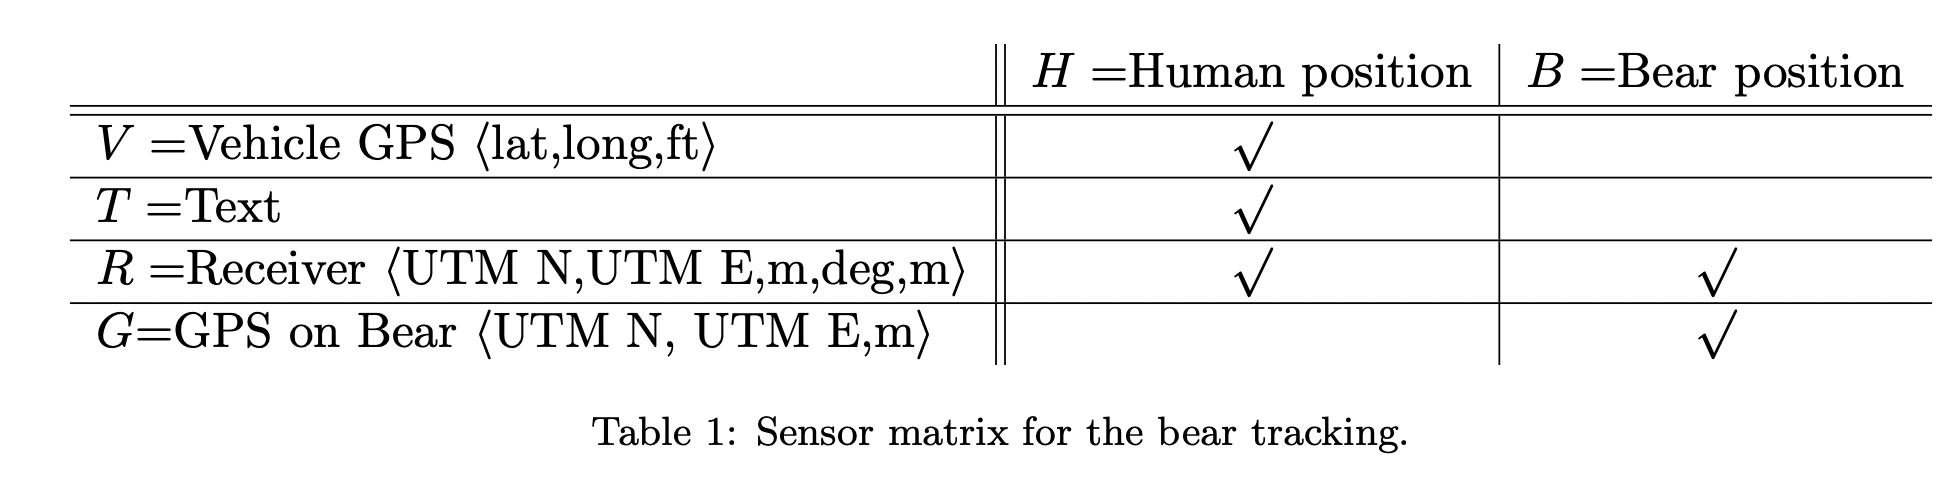
\includegraphics{GeoTable1.png}
\caption{Table 1}
\end{figure}

With Pairwise interactions X, Y, and Z = \{V, T,\}, \{V, R\}, and \{R,
T\} respectively.

\begin{figure}
\centering
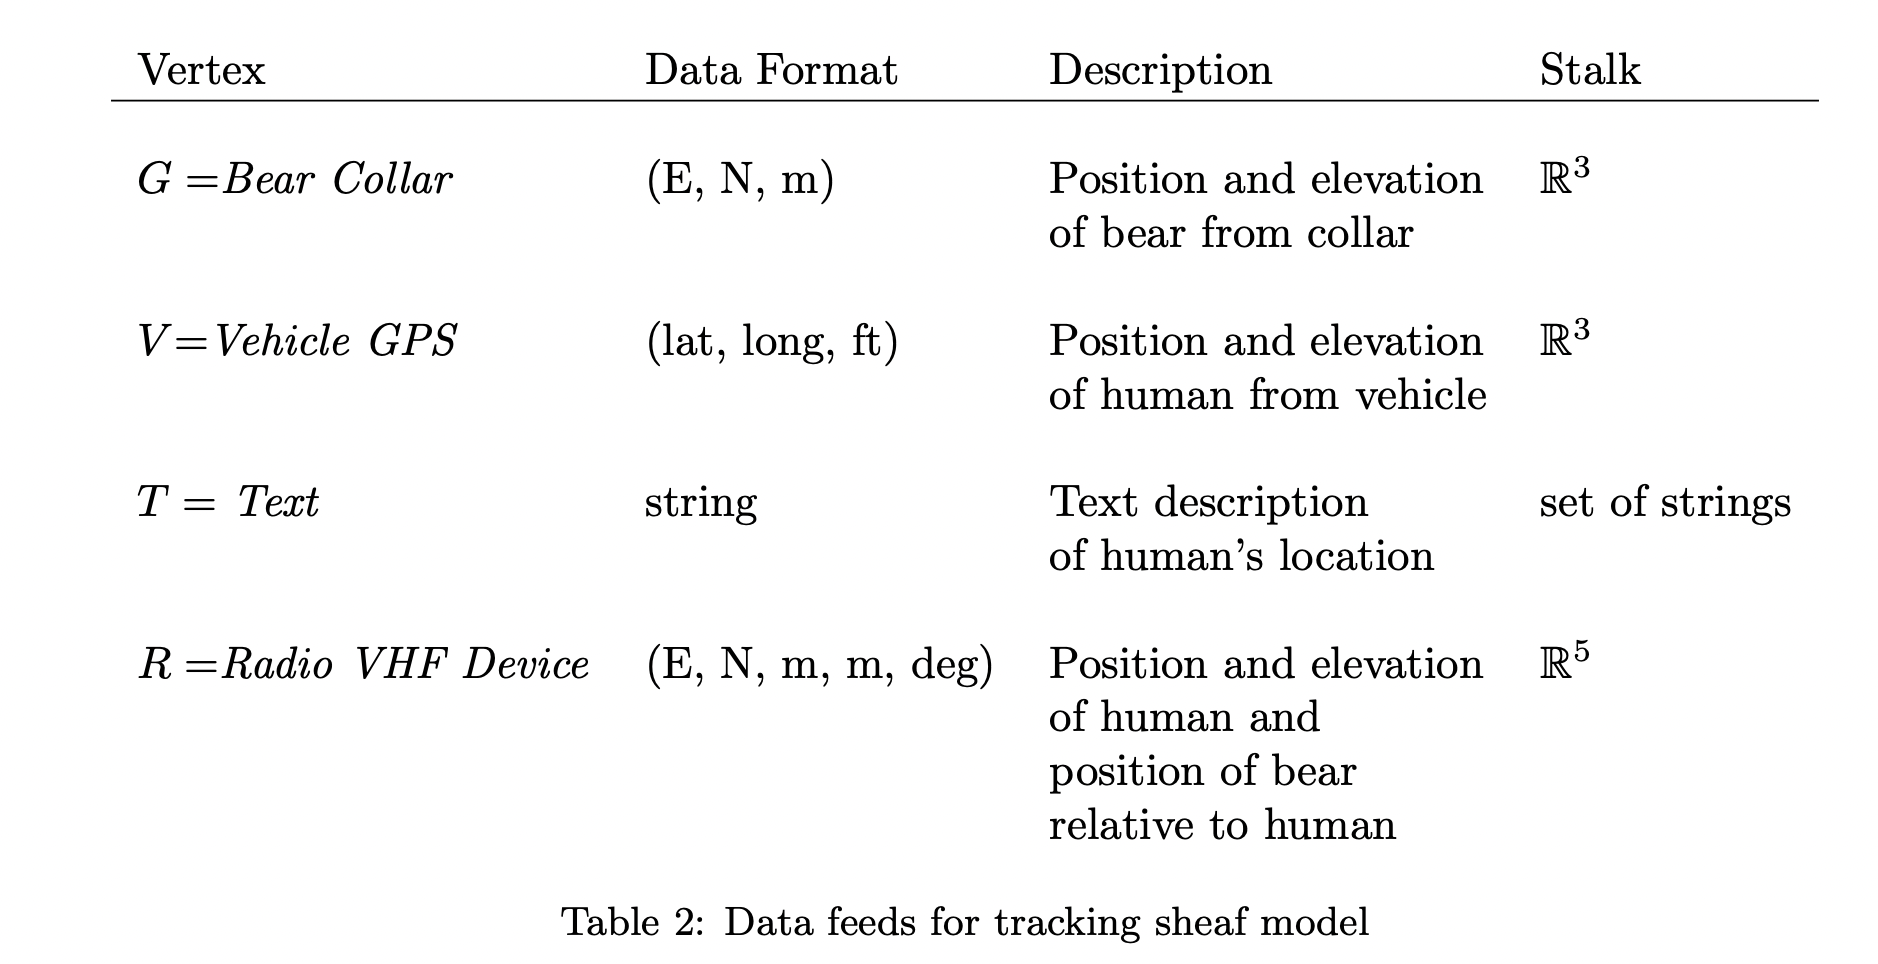
\includegraphics{GeoTable2.png}
\caption{Table 2}
\end{figure}

To convert the text descriptions we use Google Maps API {[}63{]} and to
convert the (lat, long, ft) readings, coming from the vehicle, we use
the Python open source package utm 0.4.1 {[}64{]}.

\[\phi: \mathbb{R}^5 \to \mathbb{R}^5, \phi((x, y, z, r, \theta)^T) = (x, y, z, r cos(\theta), rsin(\theta))^T  \]

\begin{figure}
\centering
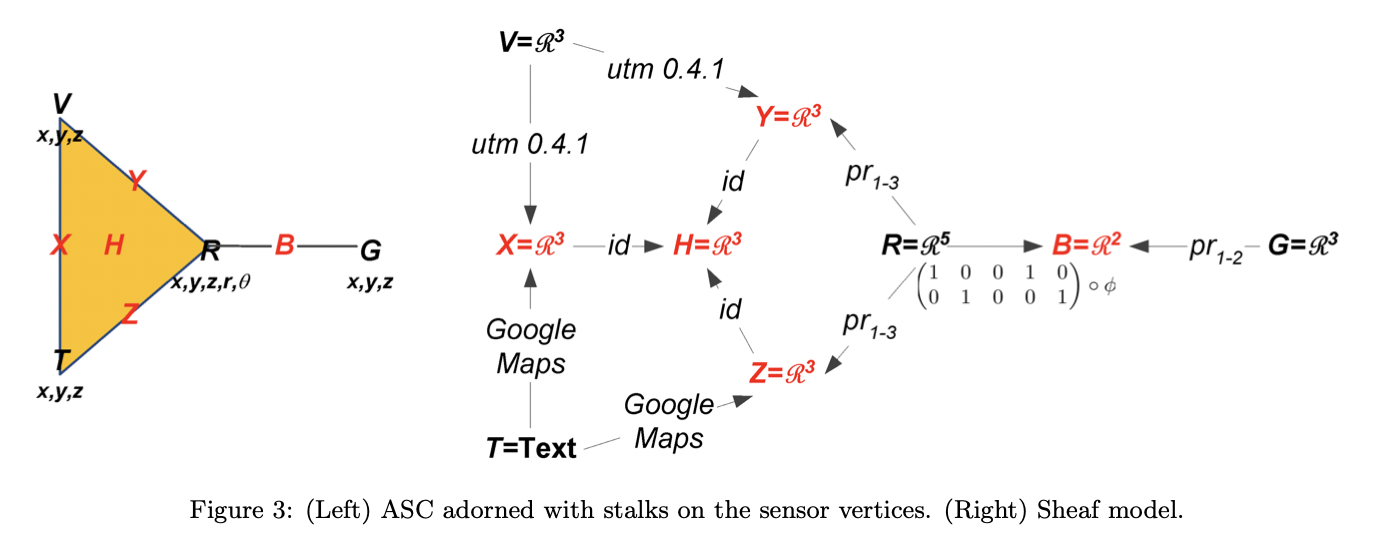
\includegraphics{GeoFigure3.png}
\caption{Figure 3}
\end{figure}

\hypertarget{update-model}{%
\section{UPDATE MODEL:}\label{update-model}}

X, Z, H -\textgreater{} R2. Z coord not available from openstreet text.
Now X, Z, H = (x, y).

\hypertarget{section}{%
\section{\texorpdfstring{\textbf{Step 1:}}{}}\label{section}}

\hypertarget{restriction-functions}{%
\subsection{Restriction Functions:}\label{restriction-functions}}

IDs \textbf{ID function return itself, refer to image for components.}

Since the pairwise relations all share UTM coordinates, only ID mappings
are needed among them -- up to the three-way H face.

In total there are 12 ID functions.

\begin{Shaded}
\begin{Highlighting}[]
\NormalTok{ID\_V }\OtherTok{\textless{}{-}} \ControlFlowTok{function}\NormalTok{(stalk)\{}
\NormalTok{  stalk }\SpecialCharTok{\%\textgreater{}\%}
    \FunctionTok{select}\NormalTok{(}\FunctionTok{c}\NormalTok{(x, y, z))}
\NormalTok{\}}
\end{Highlighting}
\end{Shaded}

\begin{Shaded}
\begin{Highlighting}[]
\NormalTok{ID\_T }\OtherTok{\textless{}{-}} \ControlFlowTok{function}\NormalTok{(stalk)\{}
\NormalTok{  stalk }\SpecialCharTok{\%\textgreater{}\%}
    \FunctionTok{select}\NormalTok{(}\FunctionTok{c}\NormalTok{(Text))}
\NormalTok{\}}
\end{Highlighting}
\end{Shaded}

\begin{Shaded}
\begin{Highlighting}[]
\NormalTok{ID\_R }\OtherTok{\textless{}{-}} \ControlFlowTok{function}\NormalTok{(stalk)\{}
\NormalTok{  stalk }\SpecialCharTok{\%\textgreater{}\%}
    \FunctionTok{select}\NormalTok{(}\FunctionTok{c}\NormalTok{(x, y, z, r, theta))}
\NormalTok{\}}
\end{Highlighting}
\end{Shaded}

\begin{Shaded}
\begin{Highlighting}[]
\NormalTok{ID\_G }\OtherTok{\textless{}{-}} \ControlFlowTok{function}\NormalTok{(stalk)\{}
\NormalTok{  stalk }\SpecialCharTok{\%\textgreater{}\%}
    \FunctionTok{select}\NormalTok{(}\FunctionTok{c}\NormalTok{(x, y, z))}
\NormalTok{\}}
\end{Highlighting}
\end{Shaded}

\begin{Shaded}
\begin{Highlighting}[]
\NormalTok{ID\_X }\OtherTok{\textless{}{-}} \ControlFlowTok{function}\NormalTok{(stalk)\{}
\NormalTok{  stalk }\SpecialCharTok{\%\textgreater{}\%}
    \FunctionTok{select}\NormalTok{(}\FunctionTok{c}\NormalTok{(x, y))}
\NormalTok{\}}
\end{Highlighting}
\end{Shaded}

\begin{Shaded}
\begin{Highlighting}[]
\NormalTok{ID\_Y }\OtherTok{\textless{}{-}} \ControlFlowTok{function}\NormalTok{(stalk)\{}
\NormalTok{  stalk }\SpecialCharTok{\%\textgreater{}\%}
    \FunctionTok{select}\NormalTok{(}\FunctionTok{c}\NormalTok{(x, y, z))}
\NormalTok{\}}
\end{Highlighting}
\end{Shaded}

\begin{Shaded}
\begin{Highlighting}[]
\NormalTok{ID\_Z }\OtherTok{\textless{}{-}} \ControlFlowTok{function}\NormalTok{(stalk)\{}
\NormalTok{  stalk }\SpecialCharTok{\%\textgreater{}\%}
    \FunctionTok{select}\NormalTok{(}\FunctionTok{c}\NormalTok{(x, y))}
\NormalTok{\}}
\end{Highlighting}
\end{Shaded}

\begin{Shaded}
\begin{Highlighting}[]
\NormalTok{ID\_B }\OtherTok{\textless{}{-}} \ControlFlowTok{function}\NormalTok{(stalk)\{}
\NormalTok{  stalk }\SpecialCharTok{\%\textgreater{}\%}
    \FunctionTok{select}\NormalTok{(}\FunctionTok{c}\NormalTok{(x, y))}
\NormalTok{\}}
\end{Highlighting}
\end{Shaded}

\begin{Shaded}
\begin{Highlighting}[]
\NormalTok{ID\_H }\OtherTok{\textless{}{-}} \ControlFlowTok{function}\NormalTok{(stalk)\{}
\NormalTok{  stalk }\SpecialCharTok{\%\textgreater{}\%}
    \FunctionTok{select}\NormalTok{(}\FunctionTok{c}\NormalTok{(x, y)) }
\NormalTok{\}}
\end{Highlighting}
\end{Shaded}

\begin{Shaded}
\begin{Highlighting}[]
\NormalTok{ID\_YH }\OtherTok{\textless{}{-}} \ControlFlowTok{function}\NormalTok{(stalk)\{}
\NormalTok{  stalk }\SpecialCharTok{\%\textgreater{}\%}
    \FunctionTok{select}\NormalTok{(}\FunctionTok{c}\NormalTok{(x, y)) }
\NormalTok{\}}
\end{Highlighting}
\end{Shaded}

\begin{Shaded}
\begin{Highlighting}[]
\NormalTok{ID\_ZH }\OtherTok{\textless{}{-}} \ControlFlowTok{function}\NormalTok{(stalk)\{}
\NormalTok{  stalk }\SpecialCharTok{\%\textgreater{}\%}
    \FunctionTok{select}\NormalTok{(}\FunctionTok{c}\NormalTok{(x, y)) }
\NormalTok{\}}
\end{Highlighting}
\end{Shaded}

\begin{Shaded}
\begin{Highlighting}[]
\NormalTok{ID\_XH }\OtherTok{\textless{}{-}} \ControlFlowTok{function}\NormalTok{(stalk)\{}
\NormalTok{  stalk }\SpecialCharTok{\%\textgreater{}\%}
    \FunctionTok{select}\NormalTok{(}\FunctionTok{c}\NormalTok{(x, y)) }
\NormalTok{\}}
\end{Highlighting}
\end{Shaded}

UTM 0.4.1 functions

For reference on the string specification being out of date:
\url{https://inbo.github.io/tutorials/tutorials/spatial_crs_coding/}

\begin{Shaded}
\begin{Highlighting}[]
\NormalTok{UTM\_VX }\OtherTok{\textless{}{-}} \ControlFlowTok{function}\NormalTok{(stalk)\{}
\NormalTok{  coordsNA }\OtherTok{\textless{}{-}} \FunctionTok{c}\NormalTok{() }\CommentTok{\# init matrix}
\NormalTok{  coordsNA}\SpecialCharTok{$}\NormalTok{x }\OtherTok{\textless{}{-}} \FunctionTok{as.numeric}\NormalTok{(stalk}\SpecialCharTok{$}\NormalTok{long) }\CommentTok{\#base r matrix gets info from order inputted not names}
\NormalTok{  coordsNA}\SpecialCharTok{$}\NormalTok{y }\OtherTok{\textless{}{-}} \FunctionTok{as.numeric}\NormalTok{(stalk}\SpecialCharTok{$}\NormalTok{lat)}
  \FunctionTok{SpatialPoints}\NormalTok{(coordsNA, }\AttributeTok{proj4string =} \FunctionTok{CRS}\NormalTok{(}\StringTok{"+proj=longlat +datum=WGS84"}\NormalTok{)) }\OtherTok{{-}\textgreater{}}\NormalTok{ llcoords }\CommentTok{\# makes s4}
  \FunctionTok{spTransform}\NormalTok{(llcoords, }\FunctionTok{CRS}\NormalTok{(}\StringTok{"+proj=utm +zone=17 +datum=WGS84 +units=m"}\NormalTok{)) }\OtherTok{{-}\textgreater{}}\NormalTok{ tcoords}
  \FunctionTok{tibble}\NormalTok{(}\AttributeTok{x =}\NormalTok{ tcoords}\SpecialCharTok{$}\NormalTok{x, }\AttributeTok{y =}\NormalTok{ tcoords}\SpecialCharTok{$}\NormalTok{y, }\AttributeTok{z =}\NormalTok{ stalk}\SpecialCharTok{$}\NormalTok{z}\SpecialCharTok{*}\FloatTok{0.3048}\NormalTok{)}
\NormalTok{\} }
\end{Highlighting}
\end{Shaded}

\begin{Shaded}
\begin{Highlighting}[]
\NormalTok{UTM\_VY }\OtherTok{\textless{}{-}} \ControlFlowTok{function}\NormalTok{(stalk)\{}
\NormalTok{  coordsNA }\OtherTok{\textless{}{-}} \FunctionTok{c}\NormalTok{() }\CommentTok{\# init matrix}
\NormalTok{  coordsNA}\SpecialCharTok{$}\NormalTok{x }\OtherTok{\textless{}{-}} \FunctionTok{as.numeric}\NormalTok{(stalk}\SpecialCharTok{$}\NormalTok{long) }\CommentTok{\#base r matrix gets info from order inputted not names}
\NormalTok{  coordsNA}\SpecialCharTok{$}\NormalTok{y }\OtherTok{\textless{}{-}} \FunctionTok{as.numeric}\NormalTok{(stalk}\SpecialCharTok{$}\NormalTok{lat)}
  \FunctionTok{SpatialPoints}\NormalTok{(coordsNA, }\AttributeTok{proj4string =} \FunctionTok{CRS}\NormalTok{(}\StringTok{"+proj=longlat +datum=WGS84"}\NormalTok{)) }\OtherTok{{-}\textgreater{}}\NormalTok{ llcoords }\CommentTok{\# makes s4}
  \FunctionTok{spTransform}\NormalTok{(llcoords, }\FunctionTok{CRS}\NormalTok{(}\StringTok{"+proj=utm +zone=17 +datum=WGS84 +units=m"}\NormalTok{)) }\OtherTok{{-}\textgreater{}}\NormalTok{ tcoords}
  \FunctionTok{tibble}\NormalTok{(}\AttributeTok{x =}\NormalTok{ tcoords}\SpecialCharTok{$}\NormalTok{x, }\AttributeTok{y =}\NormalTok{ tcoords}\SpecialCharTok{$}\NormalTok{y, }\AttributeTok{z =}\NormalTok{ stalk}\SpecialCharTok{$}\NormalTok{z}\SpecialCharTok{*}\FloatTok{0.3048}\NormalTok{)}
\NormalTok{\}}
\end{Highlighting}
\end{Shaded}

Google Maps -\textgreater{} OpenStreetMap Data. For a cost free
solution, I used OpenStreetMap data instead of Google Maps API.

Feed OpenStreetMap a text, get lat long, turn to UTM:

\begin{Shaded}
\begin{Highlighting}[]
\NormalTok{textcoords }\OtherTok{\textless{}{-}} \ControlFlowTok{function}\NormalTok{(stalk, inputcity)\{ }\CommentTok{\# take in the stalk + the input city in quotes}
  
\NormalTok{  stalk }\SpecialCharTok{\%\textgreater{}\%}
    \FunctionTok{select}\NormalTok{(Text) }\OtherTok{{-}\textgreater{}}\NormalTok{ string}
  
\CommentTok{\# Need to get names of the roads only. First select the street name. }
\CommentTok{\# For example, Woodly Road. Second, select only the name, Woodly. }
  
\NormalTok{  string }\SpecialCharTok{\%\textgreater{}\%}
    \FunctionTok{str\_extract\_all}\NormalTok{(}\StringTok{\textquotesingle{}([}\SpecialCharTok{\textbackslash{}\textbackslash{}}\StringTok{w]*?}\SpecialCharTok{\textbackslash{}\textbackslash{}}\StringTok{S+).(Rd|Road|St|Hwy|Highway|Dr|Ln|Lane|Ct|Court|Ave|Pl)\textquotesingle{}}\NormalTok{) }\SpecialCharTok{\%\textgreater{}\%} 
    \FunctionTok{unlist}\NormalTok{()}\SpecialCharTok{\%\textgreater{}\%}
    \FunctionTok{str\_extract\_all}\NormalTok{(}\StringTok{\textquotesingle{}}\SpecialCharTok{\textbackslash{}\textbackslash{}}\StringTok{b(?!(Rd|Road|St|Hwy|Highway|Dr|Ln|Lane|Ct|Court|Ave|Pl)}\SpecialCharTok{\textbackslash{}\textbackslash{}}\StringTok{b)}\SpecialCharTok{\textbackslash{}\textbackslash{}}\StringTok{w+\textquotesingle{}}\NormalTok{) }\OtherTok{{-}\textgreater{}}\NormalTok{ names}
  
  \CommentTok{\#readline(prompt = "Enter City in Quotes: ") {-}\textgreater{} inputcity}
  \FunctionTok{print}\NormalTok{(inputcity) }\CommentTok{\# checkpt}
\NormalTok{  city }\OtherTok{\textless{}{-}} \FunctionTok{getbb}\NormalTok{(inputcity) }\CommentTok{\# get bounding box for city.}
  \CommentTok{\#head(city) \#checkpt}
  
\CommentTok{\# Check database for the road. get sf object.}
\NormalTok{  citystreets }\OtherTok{\textless{}{-}}\NormalTok{ city }\SpecialCharTok{\%\textgreater{}\%}
    \FunctionTok{opq}\NormalTok{() }\SpecialCharTok{\%\textgreater{}\%}
    \FunctionTok{add\_osm\_feature}\NormalTok{(}\StringTok{"highway"}\NormalTok{, }\FunctionTok{c}\NormalTok{(}\StringTok{"motorway"}\NormalTok{, }\StringTok{"primary"}\NormalTok{, }\StringTok{"secondary"}\NormalTok{, }\StringTok{"tertiary"}\NormalTok{, }\StringTok{"residential"}\NormalTok{,}\StringTok{"living\_street"}\NormalTok{,}\StringTok{"unclassified"}\NormalTok{, }\StringTok{"service"}\NormalTok{, }\StringTok{"footway"}\NormalTok{)) }\SpecialCharTok{\%\textgreater{}\%}
    \FunctionTok{osmdata\_sf}\NormalTok{()}
  
  \FunctionTok{print}\NormalTok{(citystreets) }\CommentTok{\#checkpt, non{-}zero?}

  \CommentTok{\#find coordinates of the first road}
  \FunctionTok{tibble}\NormalTok{(}\AttributeTok{name =}\NormalTok{ citystreets}\SpecialCharTok{$}\NormalTok{osm\_lines}\SpecialCharTok{$}\NormalTok{name, }\AttributeTok{geometry =}\NormalTok{ citystreets}\SpecialCharTok{$}\NormalTok{osm\_lines}\SpecialCharTok{$}\NormalTok{geometry) }\SpecialCharTok{\%\textgreater{}\%} \CommentTok{\# geometries are linestring objects}
    \FunctionTok{filter}\NormalTok{(}\FunctionTok{grepl}\NormalTok{(names[[}\DecValTok{1}\NormalTok{]], name)) }\SpecialCharTok{\%\textgreater{}\%}
    \FunctionTok{mutate}\NormalTok{(}\AttributeTok{points =} \FunctionTok{map}\NormalTok{(geometry, }\SpecialCharTok{\textasciitilde{}}\FunctionTok{st\_coordinates}\NormalTok{(.) }\SpecialCharTok{\%\textgreater{}\%} \FunctionTok{as.data.frame}\NormalTok{())) }\SpecialCharTok{\%\textgreater{}\%} \CommentTok{\# retrieve coordinates in matrix form}
    \FunctionTok{unnest}\NormalTok{(points)}\OtherTok{{-}\textgreater{}}\NormalTok{ geompoints\_rd1 }\CommentTok{\# coords to match}
  \FunctionTok{print}\NormalTok{(geompoints\_rd1)}
  
  \CommentTok{\# find coordinates of the second road}
  \FunctionTok{tibble}\NormalTok{(}\AttributeTok{name =}\NormalTok{ citystreets}\SpecialCharTok{$}\NormalTok{osm\_lines}\SpecialCharTok{$}\NormalTok{name, }\AttributeTok{geometry =}\NormalTok{ citystreets}\SpecialCharTok{$}\NormalTok{osm\_lines}\SpecialCharTok{$}\NormalTok{geometry) }\SpecialCharTok{\%\textgreater{}\%}
    \FunctionTok{filter}\NormalTok{(}\FunctionTok{grepl}\NormalTok{(names[[}\DecValTok{2}\NormalTok{]], name)) }\SpecialCharTok{\%\textgreater{}\%}
    \FunctionTok{mutate}\NormalTok{(}\AttributeTok{points =} \FunctionTok{map}\NormalTok{(geometry, }\SpecialCharTok{\textasciitilde{}}\FunctionTok{st\_coordinates}\NormalTok{(.) }\SpecialCharTok{\%\textgreater{}\%} \FunctionTok{as.data.frame}\NormalTok{())) }\SpecialCharTok{\%\textgreater{}\%}
    \FunctionTok{unnest}\NormalTok{(points)}\OtherTok{{-}\textgreater{}}\NormalTok{ geompoints\_rd2 }\CommentTok{\# coords to match }
  \FunctionTok{print}\NormalTok{(geompoints\_rd2)}
  
  \CommentTok{\# Hope that they intersect! Inner join on the intersection, which gives lat and long of street intersection. }
  \FunctionTok{inner\_join}\NormalTok{(geompoints\_rd1, geompoints\_rd2, }\AttributeTok{by =} \FunctionTok{c}\NormalTok{(}\AttributeTok{X =} \StringTok{"X"}\NormalTok{, }\AttributeTok{Y =} \StringTok{"Y"}\NormalTok{))}\SpecialCharTok{\%\textgreater{}\%} 
    \FunctionTok{select}\NormalTok{(X, Y) }\SpecialCharTok{\%\textgreater{}\%} \FunctionTok{head}\NormalTok{(}\DecValTok{1}\NormalTok{) }\SpecialCharTok{\%\textgreater{}\%}
    \FunctionTok{transmute}\NormalTok{(}\AttributeTok{lat=}\NormalTok{ Y, }\AttributeTok{long =}\NormalTok{ X)}
\NormalTok{\}}

\CommentTok{\# base test:}
\NormalTok{stalk }\OtherTok{\textless{}{-}} \FunctionTok{data.frame}\NormalTok{(}\AttributeTok{Text =} \FunctionTok{c}\NormalTok{(}\StringTok{"Intersection at Victoria Rd and Meadow Rd"}\NormalTok{))}
\NormalTok{stalk2 }\OtherTok{\textless{}{-}} \FunctionTok{data.frame}\NormalTok{(}\AttributeTok{Text =} \FunctionTok{c}\NormalTok{(}\StringTok{"Intersection of Wood Ave and Parker Road"}\NormalTok{))}
\CommentTok{\# Further testing should be done with numbered streets}

\FunctionTok{textcoords}\NormalTok{(stalk, }\StringTok{"Asheville"}\NormalTok{)}
\end{Highlighting}
\end{Shaded}

\begin{verbatim}
## [1] "Asheville"
\end{verbatim}

\begin{verbatim}
## Object of class 'osmdata' with:
##                  $bbox : 35.4164642,-82.6703643,35.6560763,-82.4604691
##         $overpass_call : The call submitted to the overpass API
##                  $meta : metadata including timestamp and version numbers
##            $osm_points : 'sf' Simple Features Collection with 207213 points
##             $osm_lines : 'sf' Simple Features Collection with 22159 linestrings
##          $osm_polygons : 'sf' Simple Features Collection with 240 polygons
##        $osm_multilines : NULL
##     $osm_multipolygons : NULL
\end{verbatim}

\begin{verbatim}
## # A tibble: 132 x 5
##    name                                               geometry     X     Y    L1
##    <chr>                                      <LINESTRING [°]> <dbl> <dbl> <dbl>
##  1 Victoria Road (-82.55106 35.57784, -82.5512 35.57773, -82.~ -82.6  35.6     1
##  2 Victoria Road (-82.55106 35.57784, -82.5512 35.57773, -82.~ -82.6  35.6     1
##  3 Victoria Road (-82.55106 35.57784, -82.5512 35.57773, -82.~ -82.6  35.6     1
##  4 Victoria Road (-82.55106 35.57784, -82.5512 35.57773, -82.~ -82.6  35.6     1
##  5 Victoria Road (-82.55106 35.57784, -82.5512 35.57773, -82.~ -82.6  35.6     1
##  6 Victoria Road (-82.55106 35.57784, -82.5512 35.57773, -82.~ -82.6  35.6     1
##  7 Victoria Road (-82.55106 35.57784, -82.55097 35.57808, -82~ -82.6  35.6     1
##  8 Victoria Road (-82.55106 35.57784, -82.55097 35.57808, -82~ -82.6  35.6     1
##  9 Victoria Road (-82.55106 35.57784, -82.55097 35.57808, -82~ -82.6  35.6     1
## 10 Victoria Road (-82.55106 35.57784, -82.55097 35.57808, -82~ -82.6  35.6     1
## # ... with 122 more rows
## # A tibble: 713 x 5
##    name                                               geometry     X     Y    L1
##    <chr>                                      <LINESTRING [°]> <dbl> <dbl> <dbl>
##  1 Brook Meadow Lane     (-82.48762 35.47852, -82.48731 35.47~ -82.5  35.5     1
##  2 Brook Meadow Lane     (-82.48762 35.47852, -82.48731 35.47~ -82.5  35.5     1
##  3 Brook Meadow Lane     (-82.48762 35.47852, -82.48731 35.47~ -82.5  35.5     1
##  4 Brook Meadow Lane     (-82.48762 35.47852, -82.48731 35.47~ -82.5  35.5     1
##  5 Mallory Meadows Court (-82.49185 35.45209, -82.49186 35.45~ -82.5  35.5     1
##  6 Mallory Meadows Court (-82.49185 35.45209, -82.49186 35.45~ -82.5  35.5     1
##  7 Mallory Meadows Court (-82.49185 35.45209, -82.49186 35.45~ -82.5  35.5     1
##  8 Mallory Meadows Court (-82.49185 35.45209, -82.49186 35.45~ -82.5  35.5     1
##  9 Mallory Meadows Court (-82.49185 35.45209, -82.49186 35.45~ -82.5  35.5     1
## 10 Mallory Meadows Court (-82.49185 35.45209, -82.49186 35.45~ -82.5  35.5     1
## # ... with 703 more rows
\end{verbatim}

\begin{verbatim}
## # A tibble: 1 x 2
##     lat  long
##   <dbl> <dbl>
## 1  35.6 -82.6
\end{verbatim}

\begin{Shaded}
\begin{Highlighting}[]
\NormalTok{OSM\_TX }\OtherTok{\textless{}{-}} \ControlFlowTok{function}\NormalTok{(stalk)\{}
\NormalTok{  stalk }\SpecialCharTok{\%\textgreater{}\%} 
    \FunctionTok{textcoords}\NormalTok{(}\StringTok{"Asheville"}\NormalTok{) }\SpecialCharTok{\%\textgreater{}\%} \CommentTok{\# pipe in stalk, then add input city, here from the paper we are in Asheville.}
    \FunctionTok{UTM\_VX}\NormalTok{()}
\NormalTok{\}}
\end{Highlighting}
\end{Shaded}

\begin{Shaded}
\begin{Highlighting}[]
\NormalTok{OSM\_TZ }\OtherTok{\textless{}{-}} \ControlFlowTok{function}\NormalTok{(stalk)\{}
\NormalTok{    stalk }\SpecialCharTok{\%\textgreater{}\%} 
    \FunctionTok{textcoords}\NormalTok{(}\StringTok{"Asheville"}\NormalTok{) }\SpecialCharTok{\%\textgreater{}\%}
    \FunctionTok{UTM\_VX}\NormalTok{()}
\NormalTok{\}}
\end{Highlighting}
\end{Shaded}

\(pr_{x-y}\): Labels of the form prx-y are projections of the
corresponding coordinates (also presentable as binary matrices of the
appropriate form).

\(pr_{1-2}\)

\begin{Shaded}
\begin{Highlighting}[]
\NormalTok{PRgb\_1\_2 }\OtherTok{\textless{}{-}} \ControlFlowTok{function}\NormalTok{(stalk)\{}
\NormalTok{  stalk }\SpecialCharTok{\%\textgreater{}\%}
    \FunctionTok{select}\NormalTok{(}\FunctionTok{c}\NormalTok{(x, y)) }
\NormalTok{\}}
\end{Highlighting}
\end{Shaded}

\(pr_{1-3}\)

\begin{Shaded}
\begin{Highlighting}[]
\NormalTok{PRry\_1\_3 }\OtherTok{\textless{}{-}} \ControlFlowTok{function}\NormalTok{(stalk)\{}
\NormalTok{  stalk }\SpecialCharTok{\%\textgreater{}\%}
    \FunctionTok{select}\NormalTok{(}\FunctionTok{c}\NormalTok{(x, y, z))}
\NormalTok{\}}
\end{Highlighting}
\end{Shaded}

\begin{Shaded}
\begin{Highlighting}[]
\NormalTok{PRrz\_1\_3 }\OtherTok{\textless{}{-}} \ControlFlowTok{function}\NormalTok{(stalk)\{}
\NormalTok{  stalk }\SpecialCharTok{\%\textgreater{}\%}
    \FunctionTok{select}\NormalTok{(}\FunctionTok{c}\NormalTok{(x, y)) }
\NormalTok{\}}
\end{Highlighting}
\end{Shaded}

``Finally, the restriction from R up to B is the composition of the
polar conversion of the final two components with the projection on the
first two to predict the bear position from the radiocollar GPS,
bearing, and range.''

\[\begin{pmatrix}
1 & 0 & 0 & 1 & 0\\
0 & 1 & 0 & 0 & 1
\end{pmatrix} \circ
\phi:(x, y, z, r cos(\theta), rsin(\theta))^T  \]

\begin{Shaded}
\begin{Highlighting}[]
\NormalTok{phi\_RB }\OtherTok{\textless{}{-}} \ControlFlowTok{function}\NormalTok{(stalk)\{}
\NormalTok{  stalk }\SpecialCharTok{\%\textgreater{}\%}
    \FunctionTok{mutate}\NormalTok{(}\AttributeTok{x =}\NormalTok{ x}\SpecialCharTok{+}\NormalTok{r}\SpecialCharTok{*}\FunctionTok{sin}\NormalTok{(theta}\SpecialCharTok{*}\NormalTok{pi}\SpecialCharTok{/}\DecValTok{180}\NormalTok{), }\AttributeTok{y =}\NormalTok{ y}\SpecialCharTok{+}\NormalTok{r}\SpecialCharTok{*}\FunctionTok{cos}\NormalTok{(theta}\SpecialCharTok{*}\NormalTok{pi}\SpecialCharTok{/}\DecValTok{180}\NormalTok{)) }\SpecialCharTok{\%\textgreater{}\%}
    \FunctionTok{select}\NormalTok{(}\FunctionTok{c}\NormalTok{(x, y))}
\NormalTok{\}}
\end{Highlighting}
\end{Shaded}

\hypertarget{section-1}{%
\section{\texorpdfstring{\textbf{Step 2:}}{}}\label{section-1}}

\hypertarget{assignment-table}{%
\subsection{Assignment Table:}\label{assignment-table}}

Global section inputs for case 1: 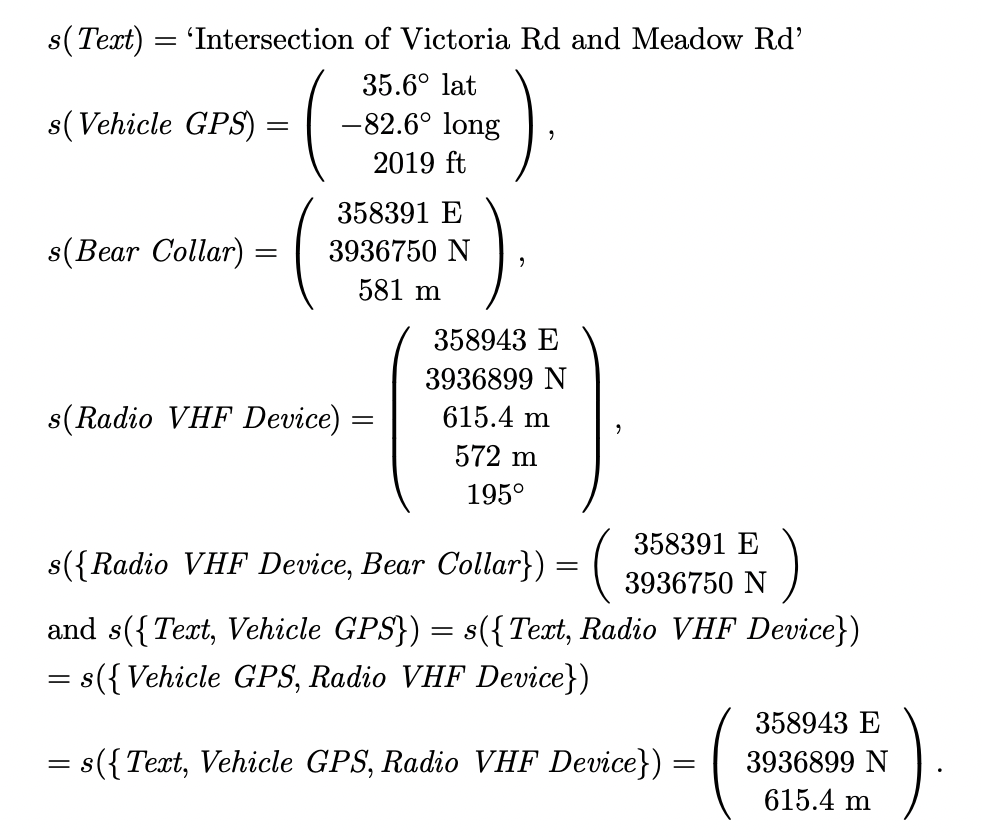
\includegraphics{GeoGlobalSect1.png}

\begin{Shaded}
\begin{Highlighting}[]
\NormalTok{Table }\OtherTok{\textless{}{-}} \FunctionTok{read.csv}\NormalTok{(}\StringTok{"GeoAssignmentTable.csv"}\NormalTok{) }
\NormalTok{Table}
\end{Highlighting}
\end{Shaded}

\begin{verbatim}
##              sensor key entity                                       case1
## 1       Bear Collar   G      x                                      358391
## 2       Bear Collar   G      y                                     3936750
## 3       Bear Collar   G      z                                         581
## 4       Vehicle GPS   V    lat                                    35.56574
## 5       Vehicle GPS   V   long                                  -82.556529
## 6       Vehicle GPS   V      z                                        2019
## 7              Text   T   Text "Intersection of Victoria Rd and Meadow Rd"
## 8  Radio VHF Device   R      x                                      358943
## 9  Radio VHF Device   R      y                                     3936899
## 10 Radio VHF Device   R      z                                       615.4
## 11 Radio VHF Device   R      r                                         572
## 12 Radio VHF Device   R  theta                                         255
## 13            Human   X      x                                      358943
## 14            Human   X      y                                     3936899
## 15            Human   X      z                                       615.4
## 16            Human   Y      x                                      358943
## 17            Human   Y      y                                     3936899
## 18            Human   Y      z                                       615.4
## 19            Human   Z      x                                      358943
## 20            Human   Z      y                                     3936899
## 21            Human   Z      z                                       615.4
## 22             Bear   B      x                                      358391
## 23             Bear   B      y                                     3936750
## 24            Human   H      x                                      358943
## 25            Human   H      y                                     3936899
## 26            Human   H      z                                       615.4
##                       case2 units
## 1                    362888     E
## 2                   3938373     N
## 3                       577     m
## 4                 35.571411   lat
## 5                -82.515491 long 
## 6                      2174    ft
## 7  "Wood Ave. at Parker Rd"  Text
## 8                    362666     E
## 9                   3937469     N
## 10                      643     m
## 11                     1500     m
## 12                       40   deg
## 13                   362666     E
## 14                  3937469     N
## 15                      643     m
## 16                   362666     E
## 17                  3937469     N
## 18                      643     m
## 19                   362666     E
## 20                  3937469     N
## 21                      643     m
## 22                   362888     E
## 23                  3938373     N
## 24                   362666     E
## 25                  3937469     N
## 26                      643     m
\end{verbatim}

\hypertarget{model}{%
\subsection{MODEL:}\label{model}}

\begin{Shaded}
\begin{Highlighting}[]
\NormalTok{model }\OtherTok{\textless{}{-}} \FunctionTok{tibble}\NormalTok{(}\AttributeTok{map =} \FunctionTok{c}\NormalTok{(ID\_V, ID\_T, ID\_R, ID\_G, ID\_X, ID\_Y, ID\_Z, ID\_B, ID\_H, UTM\_VX, UTM\_VY,phi\_RB,PRgb\_1\_2, PRry\_1\_3, PRrz\_1\_3, ID\_YH, ID\_ZH, ID\_XH, OSM\_TZ, OSM\_TX),}
                    \AttributeTok{source =} \FunctionTok{c}\NormalTok{(}\StringTok{"V"}\NormalTok{, }\StringTok{"T"}\NormalTok{, }\StringTok{"R"}\NormalTok{, }\StringTok{"G"}\NormalTok{, }\StringTok{"X"}\NormalTok{, }\StringTok{"Y"}\NormalTok{, }\StringTok{"Z"}\NormalTok{, }\StringTok{"B"}\NormalTok{, }\StringTok{"H"}\NormalTok{, }\StringTok{"V"}\NormalTok{, }\StringTok{"V"}\NormalTok{, }\StringTok{"R"}\NormalTok{, }\StringTok{"G"}\NormalTok{, }\StringTok{"R"}\NormalTok{, }\StringTok{"R"}\NormalTok{, }\StringTok{"Y"}\NormalTok{, }\StringTok{"Z"}\NormalTok{, }\StringTok{"X"}\NormalTok{, }\StringTok{"T"}\NormalTok{, }\StringTok{"T"}\NormalTok{), }\CommentTok{\#key == source}
                    \AttributeTok{dest =}   \FunctionTok{c}\NormalTok{(}\StringTok{"V"}\NormalTok{, }\StringTok{"T"}\NormalTok{, }\StringTok{"R"}\NormalTok{, }\StringTok{"G"}\NormalTok{, }\StringTok{"X"}\NormalTok{, }\StringTok{"Y"}\NormalTok{, }\StringTok{"Z"}\NormalTok{, }\StringTok{"B"}\NormalTok{, }\StringTok{"H"}\NormalTok{, }\StringTok{"X"}\NormalTok{, }\StringTok{"Y"}\NormalTok{, }\StringTok{"B"}\NormalTok{, }\StringTok{"B"}\NormalTok{, }\StringTok{"Y"}\NormalTok{, }\StringTok{"Z"}\NormalTok{, }\StringTok{"H"}\NormalTok{, }\StringTok{"H"}\NormalTok{, }\StringTok{"H"}\NormalTok{, }\StringTok{"Z"}\NormalTok{, }\StringTok{"X"}\NormalTok{))}

\FunctionTok{as.data.frame}\NormalTok{(model) }\OtherTok{{-}\textgreater{}}\NormalTok{ model }\CommentTok{\#20x11}
\CommentTok{\# Checked all sources and dests match functions √}
\end{Highlighting}
\end{Shaded}

Attach model to table, and execute functions to make full sheaf model
with outputs:

\begin{Shaded}
\begin{Highlighting}[]
\NormalTok{Table }\SpecialCharTok{\%\textgreater{}\%}
  \FunctionTok{select}\NormalTok{(entity, case1, key)}\SpecialCharTok{\%\textgreater{}\%}
  \FunctionTok{pivot\_wider}\NormalTok{(}\AttributeTok{names\_from =}\NormalTok{ entity, }\AttributeTok{values\_from =}\NormalTok{ case1)}\SpecialCharTok{\%\textgreater{}\%}
  \FunctionTok{mutate}\NormalTok{(}\FunctionTok{across}\NormalTok{(}\FunctionTok{c}\NormalTok{(x, y, z, lat, long, theta, r), as.numeric))}\SpecialCharTok{\%\textgreater{}\%} \CommentTok{\# needed to transform from chr to dbl. }
  \FunctionTok{right\_join}\NormalTok{(model, }\AttributeTok{by =} \FunctionTok{c}\NormalTok{(}\AttributeTok{key =} \StringTok{"source"}\NormalTok{)) }\SpecialCharTok{\%\textgreater{}\%}
  \FunctionTok{nest}\NormalTok{(}\AttributeTok{stalkinput =} \DecValTok{2}\SpecialCharTok{:}\DecValTok{9}\NormalTok{) }\SpecialCharTok{\%\textgreater{}\%}
  \FunctionTok{mutate}\NormalTok{(}\AttributeTok{stalkoutput =} \FunctionTok{map2}\NormalTok{(}\AttributeTok{.x=}\NormalTok{ map, }\AttributeTok{.y =}\NormalTok{ stalkinput, }\AttributeTok{.f =}\NormalTok{ exec)) }\OtherTok{{-}\textgreater{}}\NormalTok{ sheaf }\CommentTok{\# These were all global sections, should have cons.rad of 0}
\end{Highlighting}
\end{Shaded}

\begin{verbatim}
## [1] "Asheville"
\end{verbatim}

\begin{verbatim}
## Object of class 'osmdata' with:
##                  $bbox : 35.4164642,-82.6703643,35.6560763,-82.4604691
##         $overpass_call : The call submitted to the overpass API
##                  $meta : metadata including timestamp and version numbers
##            $osm_points : 'sf' Simple Features Collection with 207213 points
##             $osm_lines : 'sf' Simple Features Collection with 22159 linestrings
##          $osm_polygons : 'sf' Simple Features Collection with 240 polygons
##        $osm_multilines : NULL
##     $osm_multipolygons : NULL
\end{verbatim}

\begin{verbatim}
## # A tibble: 132 x 5
##    name                                               geometry     X     Y    L1
##    <chr>                                      <LINESTRING [°]> <dbl> <dbl> <dbl>
##  1 Victoria Road (-82.55106 35.57784, -82.5512 35.57773, -82.~ -82.6  35.6     1
##  2 Victoria Road (-82.55106 35.57784, -82.5512 35.57773, -82.~ -82.6  35.6     1
##  3 Victoria Road (-82.55106 35.57784, -82.5512 35.57773, -82.~ -82.6  35.6     1
##  4 Victoria Road (-82.55106 35.57784, -82.5512 35.57773, -82.~ -82.6  35.6     1
##  5 Victoria Road (-82.55106 35.57784, -82.5512 35.57773, -82.~ -82.6  35.6     1
##  6 Victoria Road (-82.55106 35.57784, -82.5512 35.57773, -82.~ -82.6  35.6     1
##  7 Victoria Road (-82.55106 35.57784, -82.55097 35.57808, -82~ -82.6  35.6     1
##  8 Victoria Road (-82.55106 35.57784, -82.55097 35.57808, -82~ -82.6  35.6     1
##  9 Victoria Road (-82.55106 35.57784, -82.55097 35.57808, -82~ -82.6  35.6     1
## 10 Victoria Road (-82.55106 35.57784, -82.55097 35.57808, -82~ -82.6  35.6     1
## # ... with 122 more rows
## # A tibble: 713 x 5
##    name                                               geometry     X     Y    L1
##    <chr>                                      <LINESTRING [°]> <dbl> <dbl> <dbl>
##  1 Brook Meadow Lane     (-82.48762 35.47852, -82.48731 35.47~ -82.5  35.5     1
##  2 Brook Meadow Lane     (-82.48762 35.47852, -82.48731 35.47~ -82.5  35.5     1
##  3 Brook Meadow Lane     (-82.48762 35.47852, -82.48731 35.47~ -82.5  35.5     1
##  4 Brook Meadow Lane     (-82.48762 35.47852, -82.48731 35.47~ -82.5  35.5     1
##  5 Mallory Meadows Court (-82.49185 35.45209, -82.49186 35.45~ -82.5  35.5     1
##  6 Mallory Meadows Court (-82.49185 35.45209, -82.49186 35.45~ -82.5  35.5     1
##  7 Mallory Meadows Court (-82.49185 35.45209, -82.49186 35.45~ -82.5  35.5     1
##  8 Mallory Meadows Court (-82.49185 35.45209, -82.49186 35.45~ -82.5  35.5     1
##  9 Mallory Meadows Court (-82.49185 35.45209, -82.49186 35.45~ -82.5  35.5     1
## 10 Mallory Meadows Court (-82.49185 35.45209, -82.49186 35.45~ -82.5  35.5     1
## # ... with 703 more rows
\end{verbatim}

\begin{verbatim}
## Warning: Unknown or uninitialised column: `z`.
\end{verbatim}

\begin{verbatim}
## [1] "Asheville"
\end{verbatim}

\begin{verbatim}
## Object of class 'osmdata' with:
##                  $bbox : 35.4164642,-82.6703643,35.6560763,-82.4604691
##         $overpass_call : The call submitted to the overpass API
##                  $meta : metadata including timestamp and version numbers
##            $osm_points : 'sf' Simple Features Collection with 207213 points
##             $osm_lines : 'sf' Simple Features Collection with 22159 linestrings
##          $osm_polygons : 'sf' Simple Features Collection with 240 polygons
##        $osm_multilines : NULL
##     $osm_multipolygons : NULL
\end{verbatim}

\begin{verbatim}
## # A tibble: 132 x 5
##    name                                               geometry     X     Y    L1
##    <chr>                                      <LINESTRING [°]> <dbl> <dbl> <dbl>
##  1 Victoria Road (-82.55106 35.57784, -82.5512 35.57773, -82.~ -82.6  35.6     1
##  2 Victoria Road (-82.55106 35.57784, -82.5512 35.57773, -82.~ -82.6  35.6     1
##  3 Victoria Road (-82.55106 35.57784, -82.5512 35.57773, -82.~ -82.6  35.6     1
##  4 Victoria Road (-82.55106 35.57784, -82.5512 35.57773, -82.~ -82.6  35.6     1
##  5 Victoria Road (-82.55106 35.57784, -82.5512 35.57773, -82.~ -82.6  35.6     1
##  6 Victoria Road (-82.55106 35.57784, -82.5512 35.57773, -82.~ -82.6  35.6     1
##  7 Victoria Road (-82.55106 35.57784, -82.55097 35.57808, -82~ -82.6  35.6     1
##  8 Victoria Road (-82.55106 35.57784, -82.55097 35.57808, -82~ -82.6  35.6     1
##  9 Victoria Road (-82.55106 35.57784, -82.55097 35.57808, -82~ -82.6  35.6     1
## 10 Victoria Road (-82.55106 35.57784, -82.55097 35.57808, -82~ -82.6  35.6     1
## # ... with 122 more rows
## # A tibble: 713 x 5
##    name                                               geometry     X     Y    L1
##    <chr>                                      <LINESTRING [°]> <dbl> <dbl> <dbl>
##  1 Brook Meadow Lane     (-82.48762 35.47852, -82.48731 35.47~ -82.5  35.5     1
##  2 Brook Meadow Lane     (-82.48762 35.47852, -82.48731 35.47~ -82.5  35.5     1
##  3 Brook Meadow Lane     (-82.48762 35.47852, -82.48731 35.47~ -82.5  35.5     1
##  4 Brook Meadow Lane     (-82.48762 35.47852, -82.48731 35.47~ -82.5  35.5     1
##  5 Mallory Meadows Court (-82.49185 35.45209, -82.49186 35.45~ -82.5  35.5     1
##  6 Mallory Meadows Court (-82.49185 35.45209, -82.49186 35.45~ -82.5  35.5     1
##  7 Mallory Meadows Court (-82.49185 35.45209, -82.49186 35.45~ -82.5  35.5     1
##  8 Mallory Meadows Court (-82.49185 35.45209, -82.49186 35.45~ -82.5  35.5     1
##  9 Mallory Meadows Court (-82.49185 35.45209, -82.49186 35.45~ -82.5  35.5     1
## 10 Mallory Meadows Court (-82.49185 35.45209, -82.49186 35.45~ -82.5  35.5     1
## # ... with 703 more rows
\end{verbatim}

\begin{verbatim}
## Warning: Unknown or uninitialised column: `z`.
\end{verbatim}

\begin{Shaded}
\begin{Highlighting}[]
\NormalTok{Table }\SpecialCharTok{\%\textgreater{}\%}
  \FunctionTok{select}\NormalTok{(entity, case2, key)}\SpecialCharTok{\%\textgreater{}\%}
  \FunctionTok{pivot\_wider}\NormalTok{(}\AttributeTok{names\_from =}\NormalTok{ entity, }\AttributeTok{values\_from =}\NormalTok{ case2)}\SpecialCharTok{\%\textgreater{}\%}
  \FunctionTok{mutate}\NormalTok{(}\FunctionTok{across}\NormalTok{(}\FunctionTok{c}\NormalTok{(x, y, z, lat, long, theta, r), as.numeric))}\SpecialCharTok{\%\textgreater{}\%} \CommentTok{\# needed to transform from chr to dbl. }
  \FunctionTok{right\_join}\NormalTok{(model, }\AttributeTok{by =} \FunctionTok{c}\NormalTok{(}\AttributeTok{key =} \StringTok{"source"}\NormalTok{)) }\SpecialCharTok{\%\textgreater{}\%}
  \FunctionTok{nest}\NormalTok{(}\AttributeTok{stalkinput =} \DecValTok{2}\SpecialCharTok{:}\DecValTok{9}\NormalTok{) }\SpecialCharTok{\%\textgreater{}\%}
  \FunctionTok{mutate}\NormalTok{(}\AttributeTok{stalkoutput =} \FunctionTok{map2}\NormalTok{(}\AttributeTok{.x=}\NormalTok{ map, }\AttributeTok{.y =}\NormalTok{ stalkinput, }\AttributeTok{.f =}\NormalTok{ exec)) }\OtherTok{{-}\textgreater{}}\NormalTok{ sheaf2}
\end{Highlighting}
\end{Shaded}

\begin{verbatim}
## [1] "Asheville"
\end{verbatim}

\begin{verbatim}
## Object of class 'osmdata' with:
##                  $bbox : 35.4164642,-82.6703643,35.6560763,-82.4604691
##         $overpass_call : The call submitted to the overpass API
##                  $meta : metadata including timestamp and version numbers
##            $osm_points : 'sf' Simple Features Collection with 207213 points
##             $osm_lines : 'sf' Simple Features Collection with 22159 linestrings
##          $osm_polygons : 'sf' Simple Features Collection with 240 polygons
##        $osm_multilines : NULL
##     $osm_multipolygons : NULL
\end{verbatim}

\begin{verbatim}
## # A tibble: 1,238 x 5
##    name                                               geometry     X     Y    L1
##    <chr>                                      <LINESTRING [°]> <dbl> <dbl> <dbl>
##  1 The Woods Town Homes (-82.55838 35.61296, -82.55839 35.612~ -82.6  35.6     1
##  2 The Woods Town Homes (-82.55838 35.61296, -82.55839 35.612~ -82.6  35.6     1
##  3 The Woods Town Homes (-82.55838 35.61296, -82.55839 35.612~ -82.6  35.6     1
##  4 The Woods Town Homes (-82.55838 35.61296, -82.55839 35.612~ -82.6  35.6     1
##  5 The Woods Town Homes (-82.55838 35.61296, -82.55839 35.612~ -82.6  35.6     1
##  6 South Wood Alley     (-82.51563 35.56994, -82.51564 35.570~ -82.5  35.6     1
##  7 South Wood Alley     (-82.51563 35.56994, -82.51564 35.570~ -82.5  35.6     1
##  8 South Wood Alley     (-82.51563 35.56994, -82.51564 35.570~ -82.5  35.6     1
##  9 South Wood Alley     (-82.51563 35.56994, -82.51564 35.570~ -82.5  35.6     1
## 10 South Wood Alley     (-82.51563 35.56994, -82.51564 35.570~ -82.5  35.6     1
## # ... with 1,228 more rows
## # A tibble: 55 x 5
##    name                                               geometry     X     Y    L1
##    <chr>                                      <LINESTRING [°]> <dbl> <dbl> <dbl>
##  1 Parker Road (-82.47209 35.63155, -82.47215 35.63166, -82.4~ -82.5  35.6     1
##  2 Parker Road (-82.47209 35.63155, -82.47215 35.63166, -82.4~ -82.5  35.6     1
##  3 Parker Road (-82.47209 35.63155, -82.47215 35.63166, -82.4~ -82.5  35.6     1
##  4 Parker Road (-82.47209 35.63155, -82.47215 35.63166, -82.4~ -82.5  35.6     1
##  5 Parker Road (-82.47209 35.63155, -82.47215 35.63166, -82.4~ -82.5  35.6     1
##  6 Parker Road (-82.47209 35.63155, -82.47215 35.63166, -82.4~ -82.5  35.6     1
##  7 Parker Road (-82.47209 35.63155, -82.47215 35.63166, -82.4~ -82.5  35.6     1
##  8 Parker Road (-82.47209 35.63155, -82.47215 35.63166, -82.4~ -82.5  35.6     1
##  9 Parker Road (-82.47209 35.63155, -82.47215 35.63166, -82.4~ -82.5  35.6     1
## 10 Parker Road (-82.47209 35.63155, -82.47215 35.63166, -82.4~ -82.5  35.6     1
## # ... with 45 more rows
\end{verbatim}

\begin{verbatim}
## Warning: Unknown or uninitialised column: `z`.
\end{verbatim}

\begin{verbatim}
## [1] "Asheville"
\end{verbatim}

\begin{verbatim}
## Object of class 'osmdata' with:
##                  $bbox : 35.4164642,-82.6703643,35.6560763,-82.4604691
##         $overpass_call : The call submitted to the overpass API
##                  $meta : metadata including timestamp and version numbers
##            $osm_points : 'sf' Simple Features Collection with 207213 points
##             $osm_lines : 'sf' Simple Features Collection with 22159 linestrings
##          $osm_polygons : 'sf' Simple Features Collection with 240 polygons
##        $osm_multilines : NULL
##     $osm_multipolygons : NULL
\end{verbatim}

\begin{verbatim}
## # A tibble: 1,238 x 5
##    name                                               geometry     X     Y    L1
##    <chr>                                      <LINESTRING [°]> <dbl> <dbl> <dbl>
##  1 The Woods Town Homes (-82.55838 35.61296, -82.55839 35.612~ -82.6  35.6     1
##  2 The Woods Town Homes (-82.55838 35.61296, -82.55839 35.612~ -82.6  35.6     1
##  3 The Woods Town Homes (-82.55838 35.61296, -82.55839 35.612~ -82.6  35.6     1
##  4 The Woods Town Homes (-82.55838 35.61296, -82.55839 35.612~ -82.6  35.6     1
##  5 The Woods Town Homes (-82.55838 35.61296, -82.55839 35.612~ -82.6  35.6     1
##  6 South Wood Alley     (-82.51563 35.56994, -82.51564 35.570~ -82.5  35.6     1
##  7 South Wood Alley     (-82.51563 35.56994, -82.51564 35.570~ -82.5  35.6     1
##  8 South Wood Alley     (-82.51563 35.56994, -82.51564 35.570~ -82.5  35.6     1
##  9 South Wood Alley     (-82.51563 35.56994, -82.51564 35.570~ -82.5  35.6     1
## 10 South Wood Alley     (-82.51563 35.56994, -82.51564 35.570~ -82.5  35.6     1
## # ... with 1,228 more rows
## # A tibble: 55 x 5
##    name                                               geometry     X     Y    L1
##    <chr>                                      <LINESTRING [°]> <dbl> <dbl> <dbl>
##  1 Parker Road (-82.47209 35.63155, -82.47215 35.63166, -82.4~ -82.5  35.6     1
##  2 Parker Road (-82.47209 35.63155, -82.47215 35.63166, -82.4~ -82.5  35.6     1
##  3 Parker Road (-82.47209 35.63155, -82.47215 35.63166, -82.4~ -82.5  35.6     1
##  4 Parker Road (-82.47209 35.63155, -82.47215 35.63166, -82.4~ -82.5  35.6     1
##  5 Parker Road (-82.47209 35.63155, -82.47215 35.63166, -82.4~ -82.5  35.6     1
##  6 Parker Road (-82.47209 35.63155, -82.47215 35.63166, -82.4~ -82.5  35.6     1
##  7 Parker Road (-82.47209 35.63155, -82.47215 35.63166, -82.4~ -82.5  35.6     1
##  8 Parker Road (-82.47209 35.63155, -82.47215 35.63166, -82.4~ -82.5  35.6     1
##  9 Parker Road (-82.47209 35.63155, -82.47215 35.63166, -82.4~ -82.5  35.6     1
## 10 Parker Road (-82.47209 35.63155, -82.47215 35.63166, -82.4~ -82.5  35.6     1
## # ... with 45 more rows
\end{verbatim}

\begin{verbatim}
## Warning: Unknown or uninitialised column: `z`.
\end{verbatim}

\begin{Shaded}
\begin{Highlighting}[]
\CommentTok{\# This one should not have cons.rad of 0}

\CommentTok{\#Both cases work! Problem lies in connection for osmdata sometimes it doesnt run... not my problem.}
\end{Highlighting}
\end{Shaded}

\hypertarget{global-sections}{%
\section{Global Sections}\label{global-sections}}

Definition 3:

\begin{figure}
\centering
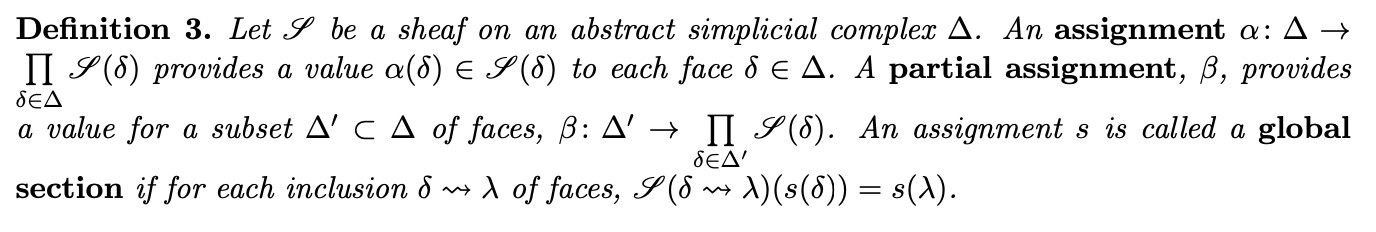
\includegraphics{GeoDef3.png}
\caption{Definition 3}
\end{figure}

***** PLEASE NOTE THAT I CANNOT FIGURE OUT DATA FOR TABLE FOR EXAMPLE
5.2\ldots, IF ITS THERE PLS HELP. *******

\hypertarget{consistency-radius}{%
\section{Consistency Radius:}\label{consistency-radius}}

******* BELOW ARE NOTES FROM SHEAFCANON, REDO FOR GEO *******

\[d_U(x,y) = \sqrt{\sum_{i \in columns} \frac{A_i}{ncol} | x_i - y_i| ^2}\]
A is the unit conversion.

We converted everything to radians.

Unit Conversions

\begin{Shaded}
\begin{Highlighting}[]
\CommentTok{\# variables: x, y, z, lat, long, theta, text, r}
\NormalTok{UnitScale }\OtherTok{\textless{}{-}} \FunctionTok{tibble}\NormalTok{(}\AttributeTok{variable =} \FunctionTok{c}\NormalTok{(}\StringTok{"x"}\NormalTok{, }\StringTok{"y"}\NormalTok{, }\StringTok{"z"}\NormalTok{, }\StringTok{"lat"}\NormalTok{, }\StringTok{"long"}\NormalTok{, }\StringTok{"theta"}\NormalTok{, }\StringTok{"Text"}\NormalTok{, }\StringTok{"r"}\NormalTok{),}
                    \CommentTok{\#scale = c(1, 1, 1, 1, 1, 1, 1, 1))}
                    \CommentTok{\#           long, lat, ft, lat, long, deg, text,meters}
                      \AttributeTok{scale =} \FunctionTok{c}\NormalTok{(}\DecValTok{1}\NormalTok{, }\DecValTok{1}\NormalTok{, }\DecValTok{1}\SpecialCharTok{/}\FloatTok{0.3048}\NormalTok{, }\DecValTok{1}\NormalTok{, }\DecValTok{1}\NormalTok{, pi}\SpecialCharTok{/}\DecValTok{180}\NormalTok{, }\DecValTok{1}\NormalTok{, }\DecValTok{1}\NormalTok{)) }\CommentTok{\# Scaling units}
\CommentTok{\# UTM IS IN METESR, SO DONT CHANGE THOSE LAT LONGS....}

\NormalTok{SensorScale }\OtherTok{\textless{}{-}}\NormalTok{ sheaf }\SpecialCharTok{\%\textgreater{}\%} \FunctionTok{count}\NormalTok{(dest) }\CommentTok{\# Scaling Sensors, by n?}
\end{Highlighting}
\end{Shaded}

\begin{Shaded}
\begin{Highlighting}[]
\CommentTok{\#Consistency Variance}
\NormalTok{sheaf }\SpecialCharTok{\%\textgreater{}\%}
  \FunctionTok{group\_by}\NormalTok{(dest) }\SpecialCharTok{\%\textgreater{}\%}
  \FunctionTok{unnest}\NormalTok{(stalkoutput)}\SpecialCharTok{\%\textgreater{}\%}
  \FunctionTok{summarise}\NormalTok{(}\FunctionTok{across}\NormalTok{(}\DecValTok{4}\SpecialCharTok{:}\DecValTok{9}\NormalTok{, }\SpecialCharTok{\textasciitilde{}} \FunctionTok{var}\NormalTok{(.,}\AttributeTok{na.rm =} \ConstantTok{TRUE}\NormalTok{)))}\SpecialCharTok{\%\textgreater{}\%} \CommentTok{\# Probs dont want var...}
  \FunctionTok{pivot\_longer}\NormalTok{(}\AttributeTok{cols =} \DecValTok{2}\SpecialCharTok{:}\DecValTok{7}\NormalTok{, }\AttributeTok{names\_to =} \StringTok{"variable"}\NormalTok{, }\AttributeTok{values\_to =} \StringTok{"stalk"}\NormalTok{) }\SpecialCharTok{\%\textgreater{}\%}
  \FunctionTok{filter}\NormalTok{(}\SpecialCharTok{!}\FunctionTok{is.na}\NormalTok{(stalk)) }\SpecialCharTok{\%\textgreater{}\%}
  \FunctionTok{left\_join}\NormalTok{(UnitScale, }\AttributeTok{by =} \FunctionTok{c}\NormalTok{(}\AttributeTok{variable =} \StringTok{"variable"}\NormalTok{))}\SpecialCharTok{\%\textgreater{}\%}
  \FunctionTok{mutate}\NormalTok{(}\AttributeTok{ScaleValue =} \FunctionTok{n}\NormalTok{()}\SpecialCharTok{*}\NormalTok{stalk}\SpecialCharTok{*}\NormalTok{scale}\SpecialCharTok{\^{}}\DecValTok{2}\NormalTok{) }\SpecialCharTok{\%\textgreater{}\%} \CommentTok{\# conversion factor applied}
  \FunctionTok{ungroup}\NormalTok{() }\SpecialCharTok{\%\textgreater{}\%}
  \FunctionTok{summarise}\NormalTok{(}\AttributeTok{ConsistVar =} \FunctionTok{sd}\NormalTok{(ScaleValue)) }\SpecialCharTok{\%\textgreater{}\%} \CommentTok{\# should be a single number.}
  \FunctionTok{sqrt}\NormalTok{()}
\end{Highlighting}
\end{Shaded}

\begin{verbatim}
## Warning in var(Text, na.rm = TRUE): NAs introduced by coercion
\end{verbatim}

\begin{verbatim}
## # A tibble: 1 x 1
##   ConsistVar
##        <dbl>
## 1       1.01
\end{verbatim}

\begin{Shaded}
\begin{Highlighting}[]
\NormalTok{sheaf }\SpecialCharTok{\%\textgreater{}\%}
  \FunctionTok{group\_by}\NormalTok{(dest) }\SpecialCharTok{\%\textgreater{}\%}
  \FunctionTok{unnest}\NormalTok{(stalkoutput) }\SpecialCharTok{\%\textgreater{}\%}
  \FunctionTok{arrange}\NormalTok{(dest) }\SpecialCharTok{\%\textgreater{}\%}
  \FunctionTok{summarise}\NormalTok{(}\FunctionTok{across}\NormalTok{(}\DecValTok{4}\SpecialCharTok{:}\DecValTok{9}\NormalTok{, }\SpecialCharTok{\textasciitilde{}} \FunctionTok{n}\NormalTok{()}\SpecialCharTok{*}\FunctionTok{var}\NormalTok{(.,}\AttributeTok{na.rm =} \ConstantTok{TRUE}\NormalTok{))) }\SpecialCharTok{\%\textgreater{}\%} \CommentTok{\# why dont we have lat long anymore.....\%\textgreater{}\%}
  \FunctionTok{pivot\_longer}\NormalTok{(}\AttributeTok{cols =} \DecValTok{2}\SpecialCharTok{:}\DecValTok{7}\NormalTok{, }\AttributeTok{names\_to =} \StringTok{"variable"}\NormalTok{, }\AttributeTok{values\_to =} \StringTok{"stalk"}\NormalTok{) }\SpecialCharTok{\%\textgreater{}\%}
  \FunctionTok{filter}\NormalTok{(}\SpecialCharTok{!}\FunctionTok{is.na}\NormalTok{(stalk)) }\SpecialCharTok{\%\textgreater{}\%}
  \FunctionTok{left\_join}\NormalTok{(UnitScale, }\AttributeTok{by =} \FunctionTok{c}\NormalTok{(}\AttributeTok{variable =} \StringTok{"variable"}\NormalTok{)) }\SpecialCharTok{\%\textgreater{}\%}
  \FunctionTok{mutate}\NormalTok{(}\AttributeTok{ScaleValue =}\NormalTok{ stalk}\SpecialCharTok{*}\NormalTok{scale}\SpecialCharTok{\^{}}\DecValTok{2}\NormalTok{)}\SpecialCharTok{\%\textgreater{}\%}
  \FunctionTok{mutate}\NormalTok{(}\FunctionTok{sqrt}\NormalTok{(ScaleValue))}\SpecialCharTok{\%\textgreater{}\%} \CommentTok{\# conversion factor applied}
  \FunctionTok{ungroup}\NormalTok{()}\SpecialCharTok{\%\textgreater{}\%}
  \FunctionTok{summarise}\NormalTok{(}\AttributeTok{ConsistSD =} \FunctionTok{sqrt}\NormalTok{(}\FunctionTok{sum}\NormalTok{(ScaleValue)))}
\end{Highlighting}
\end{Shaded}

\begin{verbatim}
## Warning in var(Text, na.rm = TRUE): NAs introduced by coercion
\end{verbatim}

\begin{verbatim}
## # A tibble: 1 x 1
##   ConsistSD
##       <dbl>
## 1      1.08
\end{verbatim}

\end{document}
